\chapter{Obesity associated genetic signatures and pathway signatures}
\label{cha:obesity_associated_genetic_signature_and_pathway_signatures}

In this chapter, the underlying biological mechanism of the obesity associated signatures from the CR data were investigated.
In doing so, the pathway genetic signatures from the \citet{Gatza2010a} study (GT) were utilised to determine which biological pathways the obesity associated genetic signatures were most similar to.
First, the direction of GT pathway associated genetic signatures were resolved, then the pathway associated metagenes were compared with the obesity associated metagenes, and lastly linear models were constructed based on the pathway metagenes and patient \gls{bmi} to predict the obesity associated metagenes.

\section{Pathway associated genetic signatures from \citet{Gatza2010a} study}
\label{sec:pathway_associated_genetic_signatures_from_gatza2010a_study}

\subsection{Ranking and normalisation methods for pathway metagenes}
\label{sub:ranking_and_normalisation_methods}

In the \citet{Gatza2010a} study, their data comprised of samples from different studies which were aggregated into a single data set that was \gls{mas} normalised, and the metagene scores were transformed to a scale between 0 to 1 using a probit function.
However, the analyses so far have used the \gls{rma} normalisation method and ranked based on the number of samples present in the data (fractional ranking; \cref{sub:ranking_of_the_metagene_scores}).
To decide which normalisation methods or ranking approaches were suitable for the analysis, the different methods were compared in the GT data (\cref{sec:ranking_method_for_the_pathway_associated_genetic_signatures,sec:normalisation_method_for_pathway_associated_genetic_signature_transformation_matrices}).
Results shown in \cref{sec:ranking_method_for_the_pathway_associated_genetic_signatures} clarified that there was no substantive difference in the ranking approaches used.

Scatter plots were generated and the correlations were calculated for each of the GT pathway metagenes derived from either \gls{rma} or \gls{mas} normalised GT data (\cref{sec:normalisation_method_for_pathway_associated_genetic_signature_transformation_matrices}).
The GT pathway metagenes were generated using the transformation matrices that were derived from either the \gls{rma} or \gls{mas} normalised GT data.
From these results, it was clear the normalisation methods used on the data set had the most significant effect on the resulting metagenes, rather than the normalisation methods used to generate the transformation matrices (\cref{sec:normalisation_method_for_pathway_associated_genetic_signature_transformation_matrices}).
This meant that all of the data sets had to be normalised with a single normalisation method, so \gls{rma} was chosen as the normalisation method to be used as this method is regarded as being more reliable than the \gls{mas} method \citep{Irizarry2003}.

Another thing noted from these scatter plots was that there were some pathway signatures that were more variable than the others (\cref{sec:normalisation_method_for_pathway_associated_genetic_signature_transformation_matrices}).
As an example, the \gls{tgfb} metagenes were significantly more dispersed compared to the \gls{pr} metagenes, even though both of these metagenes were generated in the same data set through similar processes (\cref{fig:gt_rma_vs_mas}).
These differences were seen in other data sets as well (\cref{fig:appendix/gt_meta_rma_mas_other_data}).
This result provided evidence that some of the pathway genetic signatures from the \citet{Gatza2010a} study were less variable across different data sets than the others.
Taken together, it was decided that the GT data set should be batch corrected first (\cref{sub:batch_correction}), then normalised with the \gls{rma} method, and the metagene scores were ranked with fractional ranking (\cref{sub:ranking_of_the_metagene_scores}).

\begin{figure}[htpb]
	\centering
	\includegraphics[page=76,width=0.45\linewidth]{results2/allmeta_rma_vs_mas}
	\includegraphics[page=100,width=0.45\linewidth]{results2/allmeta_rma_vs_mas}
	\caption[Comparison of the pathway metagenes generated in the \acrshort{mas} normalised GT data set from the application of TMs, derived from either the \acrshort{rma} or \acrshort{mas} normalised GT data]{Comparison of the pathway metagenes generated in the \acrshort{mas} normalised GT data set from the application of the transformation matrices derived from either the \acrshort{rma} or \acrshort{mas} normalised GT data.
	Only the \gls{pr} (left) and the \gls{tgfb}  (right) pathway metagenes are shown.
	The scatter plots for the other pathway metagenes are shown in \cref{sec:normalisation_method_for_pathway_associated_genetic_signature_transformation_matrices}.
	}
	\label{fig:gt_rma_vs_mas}
\end{figure}

\subsection{Pathway metagene directionality}
\label{sub:pathway_metagene_directionality}

Before GT pathway metagenes were compared with the obesity associated metagenes, the direction of the GT pathway metagenes had to be checked to make sure that the metagenes were in the ``correct'' direction (\cref{sub:metagene_direction}).
The correlation of all the pathway metagenes with one another were plotted as a heatmap in \cref{fig:gatza_meta_dir}.
The most prominent group had five pathways (E2F1, \gls{pi3k}, Myc, \gls{bcat} and Ras) that clustered at the top right hand corner of the heatmap.
Other groups included \gls{ifna}/\gls{ifny}/\gls{tnfa} pathways, \gls{er}/\gls{pr}/p53 pathways and p63/\gls{her2} pathways.
In addition to these highly correlated groups, \gls{stat3}/\gls{tgfb}/Src/\gls{egfr}/Akt pathways showed little correlation with one another.
Comparing these groups with the results presented by \citet{Gatza2010a} (\cref{sec:result_from_gatza2010a_study}), the identified clusters approximately resembled the pathway groups identified in by Gatza \textit{et al.}, which confirmed that the directions of GT pathway metagenes were consistent with those used by Gatza \textit{et al.}.

\begin{figure}[htpb]
	\centering
	\includegraphics[page=15,width=0.7\linewidth]{results2/gatza_meta_trans}
	\caption[Heatmap of the Pearson correlation of all the pathway metagenes with one another in the \acrshort{rma} normalised GT data]{Heatmap showing the Pearson correlation of all the pathway metagenes from the \citet{Gatza2010a} study with one another  in the \gls{rma} normalised GT data set.
		High and low correlation were represented as red and blue, respectively, where the colours were matched with the values on the scale shown in the top left histogram.
		Refer to \cref{tab:metagene_direction} for the detailed descriptions of the abbreviations used.
		}
	\label{fig:gatza_meta_dir}
\end{figure}

To see whether the directionality of the GT pathway metagenes were being transferred across to other data sets properly, pathway metagenes were generated in other data sets with the same transformation matrices and the groupings of the metagenes were examined.
CR, FM and \gls{nzbc} data were \gls{rma} normalised and transformation matrices of the pathway genetic signatures (derived from the GT data set) were applied to the data sets.
The metagenes were plotted in a heatmap (shown in \cref{sec:correlation_of_the_gt_pathway_metagenes_in_other_cancer_data_sets}), which showed similar groupings  as seen in \cref{fig:gatza_meta_dir}.
This result confirmed that the pathway metagenes were acting similarly in all of the data sets in which the transformation matrices have been applied to.

\section{Pathway associated metagenes and obesity associated metagenes}
\label{sec:pathway_associated_metagenes_and_obesity_associated_metagenes}

Results from the previous section confirmed that the pathway metagenes from the \citet{Gatza2010a} study were in the correct directions, and that the pathway metagenes were behaving as expected in the different data sets.
Now that the directions of the pathway metagenes were established, these metagenes were ready for comparison with the obesity associated metagenes.
However, all of the pathway metagenes were derived from the GT data, whereas the majority of the obesity associated metagenes were derived from the CR data, which presents a problem in terms of deciding which data set the transformation matrices should be generated in.

\subsection{Obesity and pathway metagene transformation matrices}
\label{sub:obesity_and_pathway_metagene_transformation_matrices}

Metagenes generated from the application of \gls{svd} and metagenes generated from the transformation matrix are exactly the same if the transformation matrix is derived from the same data set.
For example, an obesity associated metagene generated from the CR data with \gls{svd} would have the same values as the metagenes generated in the CR data with the transformation matrix (where the transformation matrix was derived from CR data).
Furthermore, if the \gls{svd}-derived metagenes and transformation matrix-derived metagenes were the same (or at least similar) in a different data set, this suggests that the metagene-related biology contained in the two data sets is highly similar.
In other words, the transformation matrix can be made in either the original data set or in a different data set if there was no difference in the \gls{svd}-derived or transformation matrix-derived metagenes.

To decide which data set the transformation matrices for obesity and pathway associated genetic signatures should be generated in, the \gls{svd}- and transformation matrix(TM)-generated metagene scores were compared in all of the data sets.
As in \cref{sec:pathway_associated_genetic_signatures_from_gatza2010a_study}, all data sets were normalised with the \gls{rma} method and metagenes were ranked with fractional ranking.
TMs for the obesity associated genetic signatures were made in the CR data set and the TMs for pathway associated genetic signatures were made in the GT data set.
Metagenes for all of the obesity and pathway associated genetic signatures were generated in all of the data sets with \gls{svd} and TMs.
The Spearman correlation of the \gls{svd}-generated and TM-generated metagene scores were calculated for each genetic signatures (\cref{tab:svd_vs_tm_path,tab:svd_vs_tm_obs}).

\begin{table}[htpb]
	\centering
	\begin{threeparttable}
	\caption[Summary of the Spearman correlations of the \gls{svd}- and TM-derived pathway metagenes in the GT, CR, \gls{nzbc} and FM data sets]{Summary of the Spearman correlations of the \gls{svd}- and transformation matrix\tnote{1}-derived pathway metagenes in the GT, CR, \gls{nzbc} and FM data sets}
	\label{tab:svd_vs_tm_path}
		\begin{tabular}{lcccc}
			& GT & CR & \gls{nzbc} & FM\\
			\hline
			\hline
			\rule{0pt}{2.25ex}Akt & 1.000 & 0.5190 & 0.5900 & 0.5563 \\
			\gls{bcat}            & 1.000 & 0.9897 & 0.9977 & 0.9905 \\
			E2F1                  & 1.000 & 0.9646 & 0.8438 & 0.9193 \\
			\gls{egfr}            & 1.000 & 0.0430 & 0.3358 & 0.4040 \\
			\gls{er}              & 1.000 & 0.9978 & 0.9942 & 0.9966 \\
			\gls{her2}            & 1.000 & 0.9553 & 0.5817 & 0.9794 \\
			\gls{ifna}            & 1.000 & 0.9830 & 0.9991 & 0.9951 \\
			\gls{ifny}            & 1.000 & 0.9086 & 0.9950 & 0.9718 \\
			Myc                   & 1.000 & 0.9878 & 0.9852 & 0.9689 \\
			p53                   & 1.000 & 0.3808 & 0.9981 & 0.7923 \\
			p63                   & 1.000 & 0.8319 & 0.2951 & 0.8368 \\
			\gls{pi3k}            & 1.000 & 0.9543 & 0.5989 & 0.9365 \\
			\gls{pr}              & 1.000 & 0.9511 & 0.9887 & 0.9845 \\
			Ras                   & 1.000 & 0.9078 & 0.9125 & 0.7229 \\
			Src                   & 1.000 & 0.9575 & 0.7173 & 0.9548 \\
			\gls{stat3}           & 1.000 & 0.1902 & 0.9159 & 0.6167 \\
			\gls{tgfb}            & 1.000 & 0.9918 & 0.2543 & 0.9890 \\
			\gls{tnfa}            & 1.000 & 0.6046 & 0.9365 & 0.4315 \\
			\hline
			\hline
		\end{tabular}
		\begin{tablenotes}
			\begin{footnotesize}
				\item [1] Transformation matrices were derived from the \gls{rma} normalised GT data set.
			\end{footnotesize}
		\end{tablenotes}
	\end{threeparttable}
\end{table}

\begin{table}[htpb]
	\centering
	\begin{threeparttable}
	\caption[Summary of the Spearman correlations of the \gls{svd}- and TM-derived obesity metagenes in the GT, CR, \gls{nzbc} and FM data sets]{Summary of the Spearman correlations of the \gls{svd}- and transformation matrix\tnote{1}-derived obesity metagenes in the GT, CR, \gls{nzbc} and FM data sets}
		\label{tab:svd_vs_tm_obs}
		\begin{tabular}{lcccc}
			& CR & GT & FM & \gls{nzbc}\\
			\hline
			\hline
			\rule{0pt}{2.25ex} Cr & 1.000     & 0.9985 & 0.9872 & 0.9161 \\
			Res                   & 1.000     & 0.9987 & 0.9898 & 0.9652 \\
			CrOl                  & 1.000     & 0.9982 & 0.9926 & 0.9715 \\
			ResOl                 & 1.000     & 0.9981 & 0.9927 & 0.9571 \\
			Ca                    & 1.000     & 0.9985 & 0.9893 & 0.9468 \\
			CaRes                 & 1.000     & 0.9988 & 0.9939 & 0.9865 \\
			CaOl                  & 1.000     & 0.9983 & 0.9937 & 0.9677 \\
			CaResOl               & 1.000     & 0.9984 & 0.9952 & 0.9642 \\
			Original              & 1.000     & 0.9928 & 0.9862 & 0.9344 \\
			\hline
			\hline
		\end{tabular}
			\begin{tablenotes}
				\begin{footnotesize}
				\item [1] Transformation matrices were derived from the \gls{rma} normalised CR data set.
				\end{footnotesize}
			\end{tablenotes}
	\end{threeparttable}
\end{table}

In \cref{tab:svd_vs_tm_path,tab:svd_vs_tm_obs}, the obesity and pathway associated genetic signatures had a correlation of 1 in CR and GT data sets respectively, as the obesity and pathway TMs were generated in the CR and GT data sets, respectively.
The correlations of the obesity and pathway metagenes were variable across different data sets, which was as expected since all the data sets were different from one another.
However, what was unexpected was the fact that there were some pathway genetic signatures that were highly correlated in all of the data sets, and there were others that varied considerably across different data sets.
For example, the \gls{bcat} pathway metagene was highly correlated in all of the data sets (\textgreater{} 0.98), whereas the \gls{stat3} pathway metagene was variable across different data sets, ranging from 0.1902 to 0.9159 (\cref{tab:svd_vs_tm_path}; \cref{sec:comparison_of_the_correlation_of_svd_and_tm_generated_pathway_metagenes}).
The fact that some pathway associated metagenes were consistent across different data sets suggested that some of these genetic signatures were reliable and did not depend on the data set the transformation matrices were derived from.
On the other hand, the genetic signatures that were not consistent across the data sets were likely to be dependent on the data set in which they were derived from, and therefore the transformation matrices for these signatures must be derived from the GT data set.
This also showed that the tumour biology may be different across the data sets, likely due to the difference in the patient cohorts that were selected for each of the studies.

In contrast to the pathway associated genetic signatures, all of the obesity associated genetic signatures showed high correlation for the \gls{svd}- and transformation matrix-generated metagenes across the different data sets.
This suggested that the obesity associated genetic signatures were relatively consistent across all data sets, and the transformation matrices for these signatures could be made in any of the data sets.
For simplicity, it was decided that the transformation matrices for all the genetic  signatures would be made in the GT data set, since there were some pathway associated signatures that were specific to the GT data.

\subsection{Comparison of the obesity and pathway associated signatures}
\label{sub:comparison_of_the_obesity_and_pathway_associated_signatures}

To visually determine which pathway associated genetic signatures were most similar to the obesity associated genetic signatures, heatmaps were created with the metagenes for all of the genetic signatures.
The directions of the pathway associated metagenes have already been determined in \cref{sec:pathway_associated_genetic_signatures_from_gatza2010a_study}, and the directions of the obesity associated metagenes were checked in GT data set as described in \cref{sub:metagene_direction}.
All of the metagenes were created in the GT data set (normalised with \gls{rma}) using \gls{svd}, and the metagene scores were plotted in a heatmap and clustered into groups (\cref{fig:gatza_allmeta}).

\begin{figure}[htpb]
	\centering
	\includegraphics[page=15,width=0.8\linewidth]{results2/all_meta_trans}
	\caption[Heatmap of the Pearson correlation of all the pathway and obesity metagenes with one another in the \acrshort{rma}-normalised GT data]{Heatmap showing the Pearson correlation of all the pathway and obesity metagenes  with one another  in the \gls{rma}-normalised GT data set.
		High and low correlation were represented as red and blue, respectively, where the colours were matched with the values on the scale shown in the top left histogram.
		Refer to \cref{tab:metagene_direction,tab:mg_abbrev} for the detailed descriptions of the abbreviations used.
		}
	\label{fig:gatza_allmeta}
\end{figure}

In \cref{fig:gatza_allmeta}, all of the obesity associated metagenes from the CR data set cluster together into a group, but none of the pathway associated metagenes had  a strong positive correlation with the obesity metagenes.
Though the  \gls{her2} and p63 pathway metagenes were grouped next to the cluster of obesity metagenes, the similarity was at most about 0.6  (Pearson correlation; \cref{fig:gatza_allmeta}).
With that said, these obesity associated metagenes seem to have a strong negative correlation with some of the pathway associated genetic signatures, such as the Akt, \gls{er}, \gls{egfr}, \gls{pr}, p53, Src and \gls{tgfb} pathways, and this strong negative correlation was observed in the other data sets as well (\cref{sec:correlation_of_the_pathway_and_obesity_metagenes_in_other_cancer_data_sets}).
In fact,  high Or metagene scores related to lower levels of gene expression for the genes in the Or signature (\cref{fig:crmetaheat}; \cref{sec:creighton_obesity_metagene}), and therefore it could be possible that many of the genes in the Or signature (and the other obesity associated signatures from the CR data) may be positively correlated with the genes in these pathway signatures.
This suggests that the obesity associated genetic signatures from the CR data may be related to these pathway signatures, rather than the obesity phenotype of the patients.

The FM obesity associated metagene did not cluster together with the obesity metagenes from the CR data set, nor with any of the other pathway metagenes.
The fact that the FM metagene did not cluster with any of the CR metagenes showed that the signals captures by the FM metagene was different from those metagenes found in the CR data set.
Furthermore, the FM metagene did not cluster with the Akt pathway in the heatmap, even though \citet{Fuentes-Mattei2014} provided clear evidence that their metagene specifically activated the Akt/\gls{mtor} signalling pathway in a mouse model.
This may have been due to the lack of consistency of the Akt pathway signature in the different data sets (\cref{tab:svd_vs_tm_path}).
Another likely reason could be that FM genetic signature was not comprised only of the genes from the Akt pathway, but genes from the other pathways as well, and so the metagene did not cluster together with the Akt pathway signature in the heatmap.

The results in this section suggested that none of the obesity associated genetic signatures were positively correlated with any of the pathway associated genetic signatures from the \citet{Gatza2010a} study.
However, some pathway signatures were negatively correlated with the obesity associated genetic signatures, which meant that the obesity signatures were likely capturing the signals from these signatures  rather than the biological signals from the obesity phenotype of the patient.

\section{Prediction of obesity associated metagenes with pathway associated metagenes}
\label{sec:prediction_of_obesity_associated_metagene_with_pathway_associate_metagene}

To confirm the biological relationship between the obesity associated metagenes with the pathway associated metagenes from the \citet{Gatza2010a} study, linear models were created to predict the obesity metagene scores with the pathway metagene scores.
If any of the pathway metagenes were significant in the linear model, this would provide evidence that the significant pathways in the linear model were related to the obesity metagene.
Since most of the obesity metagenes were found in the CR data set, and only the CR and the \gls{nzbc} data sets had \gls{bmi} information for the patients, \gls{nzbc} data set was used as the training data set to create the linear models for obesity metagene score prediction.

\subsection{Linear model prediction in the \gls{nzbc} and CR data sets}
\label{sub:linear_model_prediction_in_the_nzbc_and_cr_data_sets}

Metagene scores used for the construction of linear models were generated from the application of the transformation matrices derived from the GT data (from \cref{sec:pathway_associated_metagenes_and_obesity_associated_metagenes}) to \gls{rma} normalised \gls{nzbc} data.
From \cref{tab:svd_vs_tm_path}, it was evident that some pathway associated genetic signatures could be variable across different data sets.
Therefore, only six pathways (\gls{bcat}, \gls{er}, \gls{ifna}, \gls{ifny}, Myc and \gls{pr}) that were ``consistent'' (correlation \textgreater{} 0.9) across all of the data sets were used to construct the linear models.

For each of the obesity metagenes identified, seven linear models were created: \gls{bmi}-only, \gls{bmi} status-only, \gls{bmi} and \gls{bmi} status, pathway metagenes-only, and the combinations of pathway metagenes with \gls{bmi} and/or \gls{bmi} status.
The only variables that showed significance in any of the models that predicted the obesity metagenes taken from the CR data set were the \gls{pr} metagene and whether the patients were obese or not (\cref{tab:lm_sig_var}).
In the model that predicted the FM metagene scores, the obesity status of the patients and Myc metagene score were significant, but the \gls{pr} metagene score was not (\cref{sec:summary_of_the_linear_models_in_nzbc_data}).

\begin{table}[htpb]
	\centering
	\caption{Description of the linear models constructed from the \gls{nzbc} data to predict the Cr obesity metagene}
	\label{tab:lm_sig_var}
	\begin{threeparttable}
		\begin{tabular}{llrr}
			Linear Model & Variables & Estimate & P-value\\
			\hline
			\hline
			\rule{0pt}{2.25ex}\gls{bmi} only                           & \gls{bmi}  & -0.0016 & 0.717\\
			\hline
			\rule{0pt}{2.25ex}\gls{bmi} status only                    & Overweight & -0.0126 & 0.871\\
                                                                       & Obese      & -0.0981 & 0.166\\
			\hline
			\rule{0pt}{2.25ex}\gls{bmi} and \gls{bmi} status           & \gls{bmi}  & 0.0109  & 0.123\\
                                                                       & Overweight & -0.0687 & 0.420\\
                                                                       & Obese      & -0.2481 & \textbf{0.040}\tnote{1}\\
			\hline
			\rule{0pt}{2.25ex}Pathways only                            & \gls{bcat} & 0.0916  & 0.677\\
                                                                       & \gls{er}   & 0.0523  & 0.834\\
                                                                       & \gls{ifna} & -0.4993 & 0.307\\
                                                                       & \gls{ifny} & 0.4224  & 0.398\\
                                                                       & Myc        & -0.0038 & 0.987\\
                                                                       & \gls{pr}   & 0.5836  & \textbf{0.016}\\
			\hline
			\rule{0pt}{2.25ex}\gls{bmi} and Pathways                   & \gls{bmi}  & -0.0024 & 0.527\\
                                                                       & \gls{bcat} & 0.1121  & 0.614\\
                                                                       & \gls{er}   & 0.0540  & 0.829\\
                                                                       & \gls{ifna} & -0.5383 & 0.276\\
                                                                       & \gls{ifny} & 0.4661  & 0.358\\
                                                                       & Myc        & 0.0168  & 0.941\\
                                                                       & \gls{pr}   & 0.5927  & \textbf{0.015}\\
			\hline
			\rule{0pt}{2.25ex}\gls{bmi} status and Pathways            & Overweight & -0.0120 & 0.864\\
                                                                       & Obese      & -0.1035 & 0.113\\
                                                                       & \gls{bcat} & 0.1495  & 0.501\\
                                                                       & \gls{er}   & 0.0326  & 0.896\\
                                                                       & \gls{ifna} & -0.6707 & 0.177\\
                                                                       & \gls{ifny} & 0.5888  & 0.245\\
                                                                       & Myc        & 0.0439  & 0.846\\
                                                                       & \gls{pr}   & 0.5799  & \textbf{0.016}\\
			\hline
			\rule{0pt}{2.25ex}\gls{bmi}, \gls{bmi} status and pathways & \gls{bmi}  & 0.0091  & 0.161\\
                                                                       & Overweight & -0.0576 & 0.455\\
                                                                       & Obese      & -0.2292 & \textbf{0.040}\\
                                                                       & \gls{bcat} & 0.1460  & 0.509\\
                                                                       & \gls{er}   & 0.0091  & 0.971\\
                                                                       & \gls{ifna} & -0.6937 & 0.161\\
                                                                       & \gls{ifny} & 0.5890  & 0.243\\
                                                                       & Myc        & 0.0263  & 0.907\\
                                                                       & \gls{pr}   & 0.5449  & \textbf{0.024}\\
			\hline
			\hline
		\end{tabular}
		\begin{tablenotes}
			\begin{footnotesize}
				\item [1] All values in bold are statistically significant (p \textless{} 0.05).
			\end{footnotesize}
		\end{tablenotes}
	\end{threeparttable}
\end{table}

The models constructed from the patient \gls{bmi}, \gls{bmi} status and/or GT pathway metagene scores confirmed that none of the pathways were significant, except for the \gls{pr} and Myc pathway metagene scores in the models for the CR metagenes and the FM metagene, respectively.
It was not surprising that the \gls{pr} pathway metagene showed significance in the models generated in \gls{nzbc} data set, as majority of the patients in the \gls{nzbc} data set were \gls{pr}$^+$ (\cref{tab:clin_summary}).
The significance of the Myc metagene in the model for FM metagene was difficult to interpret, as there was no reported association of the FM metagene with the Myc pathway by \citet{Fuentes-Mattei2014}.
\textit{MYC} is an oncogene that encodes the Myc transcription factor that, when overexpressed, disrupts various pathways that directly promote tumour growth and proliferation, and has a central role in many of the cancer hallmarks \citep{Coller2000,Hanahan2000}.
``Sustained cell proliferation'' was one of the cancer hallmarks that \citet{Fuentes-Mattei2014} had shown to be related to their obesity associated genetic signature, which could be the reason that the Myc pathway metagene showed up as a significant variable in the linear model.

Since the \gls{pr} pathway metagene showed significant association in many of the linear models, linear models were made with each of the combinations of \gls{bmi}, \gls{bmi} status and \gls{pr} pathway metagene for all of the obesity associated metagenes (\cref{tab:lm_pr_only}; \cref{sec:summary_of_the_linear_models_in_nzbc_data}).
As expected, all of the linear models showed significant contribution of the \gls{pr} metagene scores to the model for all obesity metagenes (except FM metagene; \cref{sec:summary_of_the_linear_models_in_nzbc_data}).

\begin{table}[htpb]
	\centering
	\caption[Description of the linear models constructed from the \gls{nzbc} data to predict the Cr obesity, using only the patient \gls{bmi}, \gls{bmi} status and the \acrshort{pr} pathway metagene score]{Description of the linear models constructed from the \gls{nzbc} data to predict the Cr obesity, using only the patient \gls{bmi}, \gls{bmi} status and the \gls{pr} pathway metagene score}
	\label{tab:lm_pr_only}
	\begin{threeparttable}
			\begin{tabular}{llrS}
				Linear Model & Variables & Estimate & {P-value}\\
				\hline
				\hline
				\rule{0pt}{2.25ex}\gls{pr} only                            & \gls{pr}   & 0.477  & {\bfseries \num{6.06d-7}}\tnote{1}\\
				\hline
				\rule{0pt}{2.25ex}\gls{bmi} and \gls{pr}                   & \gls{bmi}  & -0.002 & 0.586\\
                                                                           & \gls{pr}   & 0.478  & {\bfseries \num{6.35d-7}}\\
				\hline
				\rule{0pt}{2.25ex}\gls{bmi} status and \gls{pr}            & Obese      & -0.085 & 0.176\\
                                                                           & Overweight & -0.011 & 0.875\\
                                                                           & \gls{pr}   & 0.471  & {\bfseries \num{8.25d-7}}\\
				\hline
				\rule{0pt}{2.25ex}\gls{bmi}, \gls{bmi} status and \gls{pr} & \gls{bmi}  & 0.007  & 0.237\\
                                                                           & Obese      & -0.188 & 0.081\\
                                                                           & Overweight & -0.049 & 0.516\\
                                                                           & \gls{pr}   & 0.459  & {\bfseries \num{1.54d-6}}\\
				\hline
				\hline
			\end{tabular}
			\begin{tablenotes}
				\begin{footnotesize}
					\item [1] All values in bold are statistically significant (p \textless{} 0.05).
				\end{footnotesize}
			\end{tablenotes}
	\end{threeparttable}
\end{table}

To determine whether any of the linear models were able to predict the corresponding obesity metagene scores, the predicted metagene scores were generated from the models and then compared with the original scores.
The original obesity metagene scores from the \gls{nzbc} were generated from the application of TM that were derived from the \gls{rma}-normalised GT data set.
These \gls{nzbc} obesity metagene scores were then compared with the metagene scores that were predicted by the linear models (\cref{fig:predict_cris_cris}).

The predicted metagenes from all of the patient \gls{bmi}-related linear models were not significantly related to the original metagene scores in many of the obesity metagenes (\cref{fig:predict_cris_cris}; \cref{sec:summary_of_the_linear_models_in_nzbc_data}).
On the other hand, all of the predicted metagenes generated from the models that used the pathway metagene scores showed significant association with the original metagene scores (\cref{fig:predict_cris_cris}; \cref{sec:summary_of_the_linear_models_in_nzbc_data}).
% TODO: check r-squared values
However, the $R^2$ values for all of the predicted metagenes against the original metagenes were very low ($R^2$ \textless{} 0.4).
All of the plots in \cref{fig:predict_cris_cris,sec:summary_of_the_linear_models_in_nzbc_data} showed clearly that the data points in the scatter plots were highly variable, suggesting that even though the association between the predicted and the true metagene scores were statistically significant, the variables in the linear models may not be strongly associated to the obesity metagene.
Furthermore, the fact that all of the predictions made with the models that contained the \gls{pr} metagene showed greater correlation with the true metagene values suggested that most of the variations in the Cr (and other) obesity metagenes were being explained by the \gls{pr} metagene alone, and the patient \gls{bmi} contributed very little to the prediction.

\begin{figure}[htpb]
	\centering
	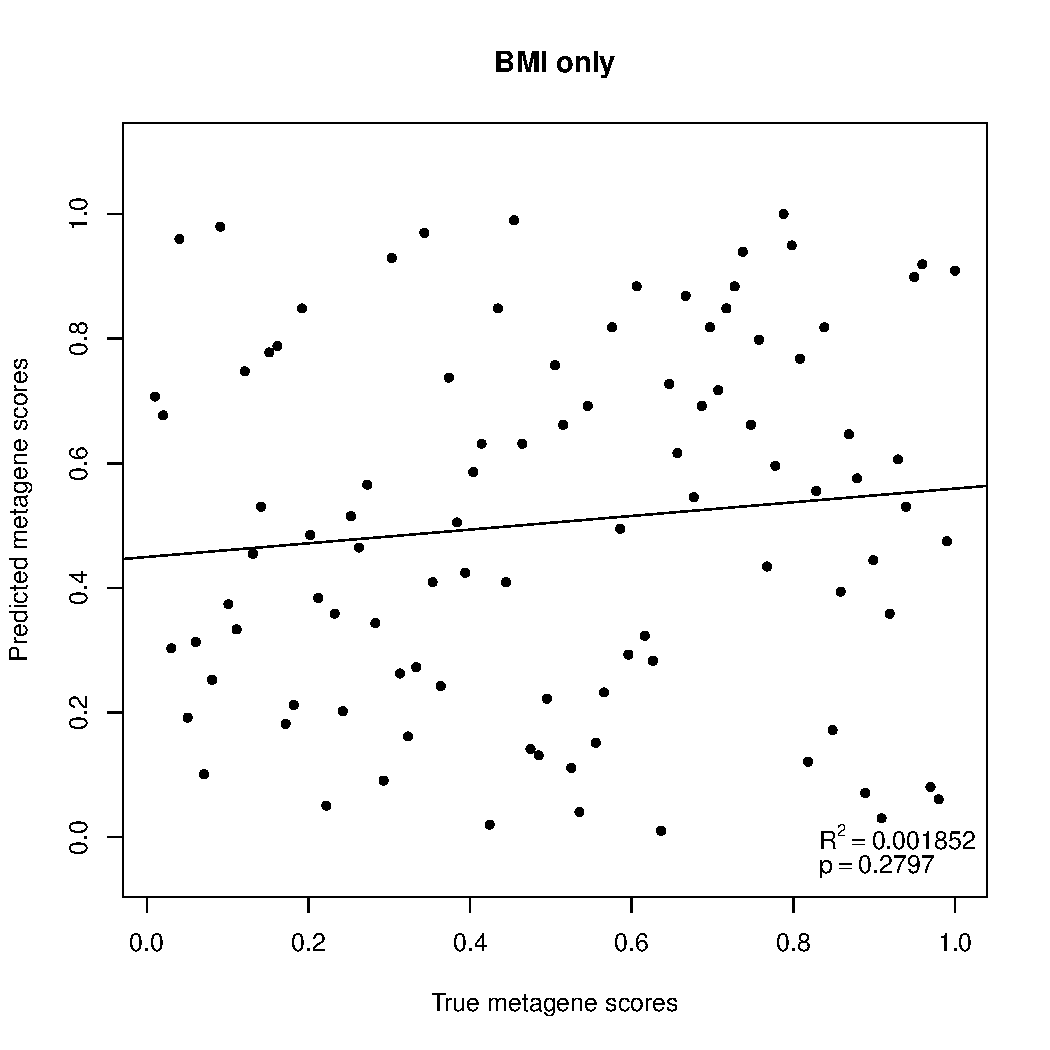
\includegraphics[page=1,width=0.32\linewidth]{results2/prediction_cris_with_cris(cris_model)}
	\includegraphics[page=2,width=0.32\linewidth]{results2/prediction_cris_with_cris(cris_model)}
	\includegraphics[page=3,width=0.32\linewidth]{results2/prediction_cris_with_cris(cris_model)}
	\includegraphics[page=4,width=0.32\linewidth]{results2/prediction_cris_with_cris(cris_model)}
	\includegraphics[page=5,width=0.32\linewidth]{results2/prediction_cris_with_cris(cris_model)}
	\includegraphics[page=6,width=0.32\linewidth]{results2/prediction_cris_with_cris(cris_model)}
	\includegraphics[page=7,width=0.32\linewidth]{results2/prediction_cris_with_cris(cris_model)}
	\includegraphics[page=74,width=0.32\linewidth]{results2/prediction_cris_with_cris(cris_model)}
	\includegraphics[page=71,width=0.32\linewidth]{results2/prediction_cris_with_cris(cris_model)}
	\includegraphics[page=72,width=0.32\linewidth]{results2/prediction_cris_with_cris(cris_model)}
	\includegraphics[page=73,width=0.32\linewidth]{results2/prediction_cris_with_cris(cris_model)}
	\caption[Comparison of the predicted Cr metagene scores with the Cr metagene score from the \gls{nzbc} data]{ Box plot and scatter plots comparing the Cr metagene score predicted by the different linear models constructed from the \gls{nzbc} data, with the Cr metagene score from the \gls{nzbc} data.
	Only the results from the models used to predict the Cr metagene scores are shown.
	The summary of the statistics for the other obesity metagene predictions from the \gls{nzbc} data are shown in \cref{sec:summary_statistics_of_the_predicted_obesity_metagenes_with_sample_bmi_bmi_status_in_nzbc_and_cr_data}.
	P-values and $R^2$-value are as described in previous figures.
	}
	\label{fig:predict_cris_cris}
\end{figure}

To confirm the results shown in the \gls{nzbc} data set (the training set), the linear models were applied to CR data (the test set).
As shown in \cref{fig:predict_cr_cris}, all of the predicted Cr metagene generated from the linear models were statistically significantly associated with the true Cr metagenes in CR data, but there were some exceptions in the models for the other obesity metagenes (\cref{sec:summary_statistics_of_the_predicted_obesity_metagenes_with_sample_bmi_bmi_status_in_nzbc_and_cr_data}).
% TODO: check r-squared values
Similar to the results from the \gls{nzbc} data set, all of the $R^2$ values were low ($R^2$ \textless{} 0.43) in the CR data set and the data points were widely spread out in the plots.
Again, these results suggested that the predicted metagene scores from the linear models may be statistically significant, but may not be relevant to the obesity metagenes which the models predict, as the predicted values were only weakly associated with the true values.

Another thing to note from \cref{fig:predict_cr_cris} was the apparent negative association of the predicted metagenes with the original metagenes in the \gls{bmi}-only, the \gls{bmi} status-only and the \gls{bmi} and \gls{bmi} status models.
One possible explanation for this was that these \gls{bmi}-based models were overfitted in the \gls{nzbc} data set, and was not generalisable in the CR data set, and thus produced negative correlations.
In fact, it was evident from the metagene analyses in \cref{cha:obesity_genetic_signatures_and_cancer} that these obesity associated genetic signatures were not generalisable with the patient \gls{bmi} in different data sets, and overfitting of the model in the \gls{nzbc} data was the likely cause of this negative correlation.

\begin{figure}[htpb]
	\centering
	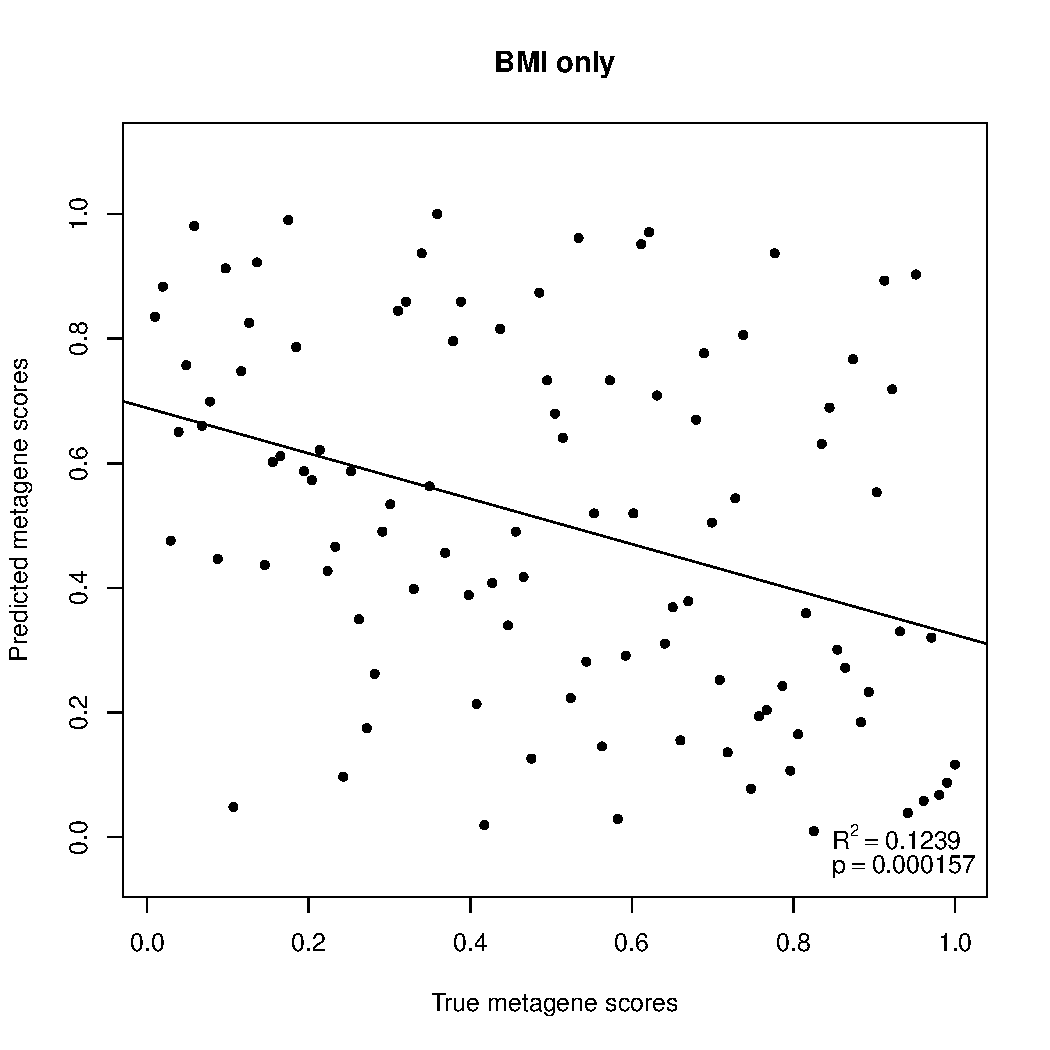
\includegraphics[page=1,width=0.32\linewidth]{results2/prediction_cr_with_cris}
	\includegraphics[page=2,width=0.32\linewidth]{results2/prediction_cr_with_cris}
	\includegraphics[page=3,width=0.32\linewidth]{results2/prediction_cr_with_cris}
	\includegraphics[page=4,width=0.32\linewidth]{results2/prediction_cr_with_cris}
	\includegraphics[page=5,width=0.32\linewidth]{results2/prediction_cr_with_cris}
	\includegraphics[page=6,width=0.32\linewidth]{results2/prediction_cr_with_cris}
	\includegraphics[page=7,width=0.32\linewidth]{results2/prediction_cr_with_cris}
	\includegraphics[page=74,width=0.32\linewidth]{results2/prediction_cr_with_cris}
	\includegraphics[page=71,width=0.32\linewidth]{results2/prediction_cr_with_cris}
	\includegraphics[page=72,width=0.32\linewidth]{results2/prediction_cr_with_cris}
	\includegraphics[page=73,width=0.32\linewidth]{results2/prediction_cr_with_cris}
	\caption[Comparison of the predicted Cr metagene scores with the Cr metagene score from the CR data]{ Box plot and scatter plots comparing the Cr metagene score predicted by the different linear models constructed from the \gls{nzbc} data, with the Cr metagene score from the CR data.
	Only the results from the models used to predict the Cr metagene scores are shown.
	The summary of the statistics for the other obesity metagene predictions from the CR data are shown in \cref{sec:summary_statistics_of_the_predicted_obesity_metagenes_with_sample_bmi_bmi_status_in_nzbc_and_cr_data}.
	P-values and $R^2$-value are as described in previous figures.
	}
	\label{fig:predict_cr_cris}
\end{figure}

\subsection{Stepwise linear model prediction in \gls{nzbc} and CR data sets}
\label{sub:stepwise_linear_model_prediction_in_nzbc_and_cr_data_sets}

Lastly, since only the six most ``consistent'' pathway metagenes were picked from a total of eighteen pathway metagene scores, linear models were constructed with all eighteen pathway metagenes in a stepwise fashion.
Step wise construction of a linear model is where the variables for a model are selected computationally depending on the contribution of the variable to the resulting linear model, and thus contain only the variables that ``matter'' to the final linear model \cref{sec:obesity_metagene_prediction_with_pathway_metagenes}.
Patient \gls{bmi}, \gls{bmi} status and all of the pathway metagenes (Akt, \gls{bcat}, E2F1, \gls{egfr}, \gls{er}, \gls{her2}, \gls{ifna}, \gls{ifny}, Myc, p53, p63, \gls{pi3k}, \gls{pr}, Ras, \gls{stat3}, Src, \gls{tgfb} and \gls{tnfa}) were used to generate the stepwise linear model for each of the obesity metagenes.
The linear models that resulted from the stepwise selection of the variables were summarised in \cref{tab:stepwise_model}.

These models were used to predict the obesity metagenes in the \gls{nzbc} data to test the performance of the models.
All of the models were able to make statistically significant prediction of the original obesity metagenes in the \gls{nzbc} data set (\cref{fig:stepwise_cris}).
% TODO: check r-squared values
Unlike the previous models, the stepwise models showed very high $R^2$ values, where most predictions had $R^2$ \textgreater{} 0.80.
The statistical significance and the strong association of the predicted metagenes were observed in the CR data set as well (\cref{fig:stepwise_cr}).
Though the $R^2$ values were slightly lower than those from the \gls{nzbc} data set, the $R^2$ values from the CR data predictions were more promising than the predictions made by the non-stepwise linear models.

\begin{ThreePartTable}
	\begin{TableNotes}
		\begin{footnotesize}
		\item [1] All values in bold are statistically significant (p \textless{} 0.05).
		\end{footnotesize}
	\end{TableNotes}
	\begin{longtable}{llr{\bfseries}S}
		\centering
		\caption[Description of the stepwise linear models constructed from the \gls{nzbc} data to predict all of the obesity metagenes]{Description of the stepwise linear models constructed from the \gls{nzbc} data to predict all of the obesity metagenes}
		\label{tab:stepwise_model}\\
			Obesity metagene & Variables retained in the model & Estimate & {P-value}\\
			\hline
		\endfirsthead
		\multicolumn{4}{c}{\tablename\ \thetable{}\ (continued)}\\
			\hline
			\hline
		\endhead
			\hline
			\hline
			Cr      & Src         & -0.1900  & \bfseries 0.005150\tnote{1}       \\
					& \gls{egfr}  & 0.1451   & \bfseries 0.002780                \\
					& \gls{tgfb}  & 0.5105   & \bfseries \num{1.17d-15}          \\
					& Akt         & -0.2821  & \bfseries \num{7.08d-06}          \\
					& \gls{ifna}  & -0.06968 & \bfseries 0.02986                 \\
			\hline
			CrOl    & Akt         & -0.3134  & \bfseries \num{1.76d-06}          \\
					& Src         & -0.5386  & \bfseries \textless{} \num{2d-16} \\
					& p53         & 0.3372   & \bfseries \num{9.18d-07}          \\
					& \gls{pr}    & -0.1115  & \bfseries 0.02760                 \\
			\hline
			Res     & \gls{tgfb}  & -0.5895  & \bfseries \num{1.53d-15}          \\
					& \gls{egfr}  & -0.3597  & \bfseries 0.0005390               \\
					& \gls{tnfa}  & 0.1604   & \bfseries 0.0006970               \\
					& \gls{bcat}  & -0.2141  & \bfseries 0.01157                 \\
					& Akt         & 0.1527   & \bfseries 0.02206                 \\
			\hline
			ResOl   & Akt         & -0.2802  & \bfseries 0.0001420               \\
					& Src         & -0.5214  & \bfseries \num{2.65d-15}          \\
					& p53         & 0.2861   & \bfseries \num{5.31d-07}          \\
			\hline
			Ca      & \gls{tgfb}  & 0.7470   & \bfseries \textless{} \num{2d-16} \\
					& Akt         & -0.2985  & \bfseries \num{2.83d-10}          \\
			\hline
			CaOl    & Src         & -0.5595  & \bfseries \num{3.88d-16}          \\
					& Akt         & -0.4331  & \bfseries \num{2.06d-11}          \\
			\hline
			CaRes   & \gls{tgfb}  & 0.7843   & \bfseries \textless{} \num{2d-16} \\
					& \gls{egfr}  & 0.2418   & \bfseries \num{2.19d-06}          \\
			\hline
			CaResOl & Src         & -0.4553  & \bfseries \num{1.57d-07}          \\
					& \gls{egfr}  & 0.2776   & \bfseries 0.0009570               \\
					& Akt         & -0.3001  & \bfseries 0.0001640               \\
					& E2F1        & 0.2484   & \bfseries 0.001300                \\
					& Myc         & 0.1584   & \bfseries 0.025220                \\
			\hline
			Or      & Src         & -0.5165  & \bfseries \textless{} \num{2d-16} \\
					& p53         & 0.3072   & \bfseries \num{2.60d-12}          \\
					& Akt         & -0.3006  & \bfseries 1.440e-07               \\
					& E2F1        & 0.09684  & \bfseries 0.01070                 \\
					& Obese       & -0.02190 & 0.2166                            \\
					& Overweight  & 0.03099  & 0.1223                            \\
			\hline
			FM      & p63         & 0.3507   & \bfseries 0.0006760               \\
					& \gls{stat3} & 0.2969   & \bfseries 0.004191                \\
					& p53         & 0.5368   & \bfseries 0.0008240               \\
					& \gls{pr}    & -0.3462  & \bfseries 0.034070                \\
			\hline
			\hline
			\insertTableNotes
	\end{longtable}
\end{ThreePartTable}

Clearly, the stepwise linear models were able to predict the obesity associated metagenes better than the models created in \cref{sub:linear_model_prediction_in_the_nzbc_and_cr_data_sets}.
This could be due to the fact that many of the stepwise linear models included many pathways that had a strong negative correlation with the obesity metagenes (Akt, \gls{er}, \gls{egfr}, \gls{pr}, p53, Src and \gls{tgfb} pathways; \cref{fig:gatza_allmeta}).
These pathway metagenes may have been better predictors of the obesity metagenes than the six pathways that were ``consistent'' across the data sets, and therefore generated better predictions than those linear models.
With that said, some of the predicted obesity metagenes from the stepwise linear models were negatively correlated with the original metagene values in the CR data (\cref{fig:stepwise_cr}).
Again, this could have been due to the model being overfit in the \gls{nzbc} data, and thus making an incorrect prediction about the obesity metagenes in the CR data.

\begin{figure}[htpb]
	\centering
	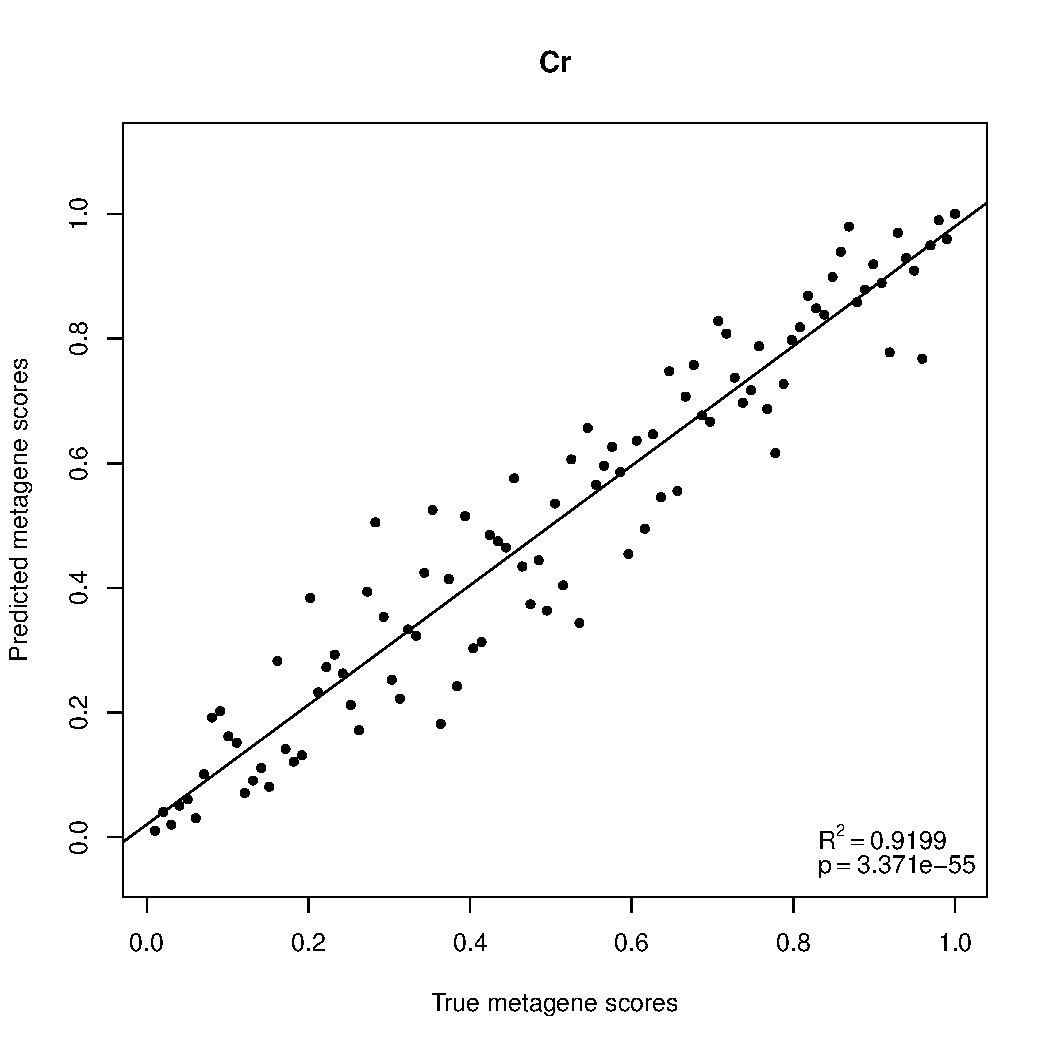
\includegraphics[page=1,width=0.32\linewidth]{results2/stepwise_cris_both_bic}
	\includegraphics[page=2,width=0.32\linewidth]{results2/stepwise_cris_both_bic}
	\includegraphics[page=3,width=0.32\linewidth]{results2/stepwise_cris_both_bic}
	\includegraphics[page=4,width=0.32\linewidth]{results2/stepwise_cris_both_bic}
	\includegraphics[page=5,width=0.32\linewidth]{results2/stepwise_cris_both_bic}
	\includegraphics[page=6,width=0.32\linewidth]{results2/stepwise_cris_both_bic}
	\includegraphics[page=7,width=0.32\linewidth]{results2/stepwise_cris_both_bic}
	\includegraphics[page=8,width=0.32\linewidth]{results2/stepwise_cris_both_bic}
	\includegraphics[page=9,width=0.32\linewidth]{results2/stepwise_cris_both_bic}
	\includegraphics[page=10,width=0.32\linewidth]{results2/stepwise_cris_both_bic}
	\caption[Comparison of all the obesity metagene scores predicted from the stepwise linear models with the original obesity metagene scores from the \gls{nzbc} data]{Scatter plots comparing all of the obesity metagene scores predicted by the stepwise linear models constructed from the \gls{nzbc} data, with the corresponding obesity metagene scores from the \gls{nzbc} data.
	P-values and $R^2$-value are as described in previous figures.}
	\label{fig:stepwise_cris}
\end{figure}

\begin{figure}[htpb]
	\centering
	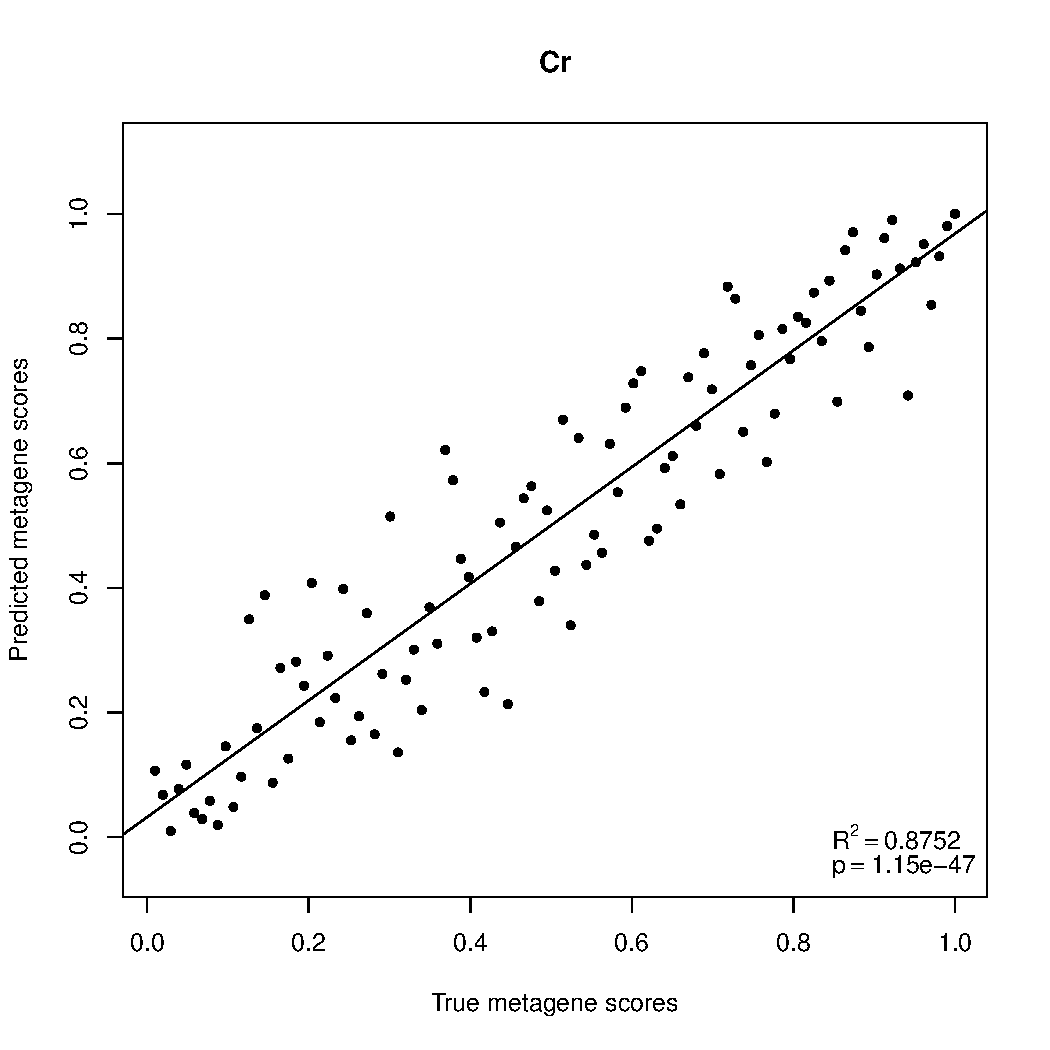
\includegraphics[page=1,width=0.32\linewidth]{results2/stepwise_cr_both_bic}
	\includegraphics[page=2,width=0.32\linewidth]{results2/stepwise_cr_both_bic}
	\includegraphics[page=3,width=0.32\linewidth]{results2/stepwise_cr_both_bic}
	\includegraphics[page=4,width=0.32\linewidth]{results2/stepwise_cr_both_bic}
	\includegraphics[page=5,width=0.32\linewidth]{results2/stepwise_cr_both_bic}
	\includegraphics[page=6,width=0.32\linewidth]{results2/stepwise_cr_both_bic}
	\includegraphics[page=7,width=0.32\linewidth]{results2/stepwise_cr_both_bic}
	\includegraphics[page=8,width=0.32\linewidth]{results2/stepwise_cr_both_bic}
	\includegraphics[page=9,width=0.32\linewidth]{results2/stepwise_cr_both_bic}
	\includegraphics[page=10,width=0.32\linewidth]{results2/stepwise_cr_both_bic}
	\caption[Comparison of all the obesity metagene scores predicted from the stepwise linear models with the original obesity metagene scores from the CR data]{Scatter plots comparing all of the obesity metagene scores predicted by the stepwise linear models constructed from the \gls{nzbc} data, with the corresponding obesity metagene scores from the CR data.
	P-values and $R^2$-value are as described in previous figures.}
	\label{fig:stepwise_cr}
\end{figure}

Taken together, these results suggest that the variables included in these stepwise models were relevant to the biology of the obesity metagenes identified in the CR and FM data sets.
However, there were no common pathways that were present in all of the models; although Akt, \gls{egfr} and Src pathway metagenes were frequently included in many of the stepwise models.
The role of the pathways included in the models and the possible biological links of these pathways to the obesity metagenes remain unclear, and should be the focus for future investigations.

